\chapter{Specyfikacja wymagań}
W tym rozdziale zawarto wymagania postawione programowi przeznaczonemu do odczytywania notacji muzycznej z~plików graficznych oraz konwersją odczytanych danych do formatu MIDI. \linebreak Najpierw zostaną przedstawione wymagania biznesowe, następnie wymagania funkcjonalne, kolejno zaś wymagania niefunkcjonalne. Rozdział zamyka słownik skrótów i~pojęć.

\section{Wymagania biznesowe}
Nazwa programu to "Photo-2-MIDI". Przeznaczeniem oprogramowania jest umożliwienie\linebreak użytkownikom zdigitalizowanie w~przystępny sposób drukowanych zapisów nutowych ze~zdjęć\linebreak lub~skanów do plików **kern oraz MIDI.

\section{Wymagania funkcjonalne}
	\begin{enumerate}
		\item Możliwość wprowadzenia plików zawierających drukowane pismo nutowe w~standardowej zachodniej notacji nutowej w~formatach PNG, JPG, PDF.
		\item Możliwość dodawania plików znajdujących się w~różnych katalogach.
		\item Możliwość usunięcia wybranego pliku z~listy plików wybranych do konwersji.
		\item Podgląd wybranych plików w~celu weryfikacji ich zawartości.
		\item Wyświetlenie powiadomienia o~zakończonej operacji konwersji.
	\end{enumerate}
	
	
\section{Wymagania niefunkcjonalne}
Program wymaga do działania:
	\begin{enumerate}
		\item Języka Python w~wersji 3.11
		\item Systemu operacyjnego Linux
		\item 2 GB wolnej pamięci operacyjnej
	\end{enumerate}
	
\section{Słownik skrótów i~pojęć}
	
\begin{enumerate}
	\item Notacja muzyczna, pismo nutowe, zapis nutowy - symboliczny język reprezentujący\linebreak odbieraną słuchowo muzykę graną na~instrumentach, czy też śpiewaną przez ludzki głos, przy pomocy symboli reprezentujących dźwięki, ich długość oraz wysokość, jak i~brak tych dźwięków\linebreak używając znaków pauz. Przy pomocy takiego języka można zapisać niemal wszystkie cechy dźwięków, takie jak rytmika, melodia, harmonia, dynamika czy artykulacja. W~tej pracy\linebreak pojęcia te będą odnosić się do nowożytnej zachodniej notacji muzycznej.
	
	\begin{figure}[htb]
		\centering
		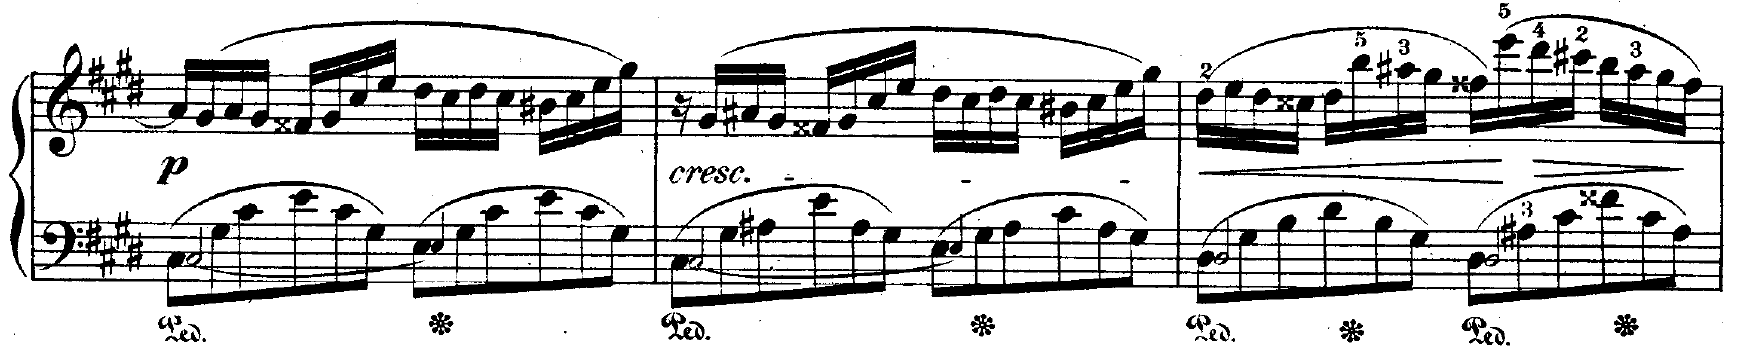
\includegraphics[width=13cm]{images/chopin_fastasie_impromtu_no_4_op_66.png}
		\caption{Fragment \textit{Fantasie-Impromptu cis-moll op. 66} Fryderyka Chopina zapisany w~nowożytnej zachodniej notacji muzycznej. }
		\label{fig:chopin_impromptu}
	\end{figure}
	
	\item format MIDI - (ang. Musical Instrument Digital Interface) popularny format plików,\linebreak który w~przeciwieństwie do standardowych formatów audio nie przenosi bezpośrednich informacji o~dźwięku, tylko informacje o~granych nutach, ich synchronizacji, trwaniu oraz głośności.
	
	\item format **kern - jeden z~najpopularniejszych cyfrowych formatów zachodniego zapisu\linebreak nutowego do komputerowej analizy muzyki
\end{enumerate}
	